\section{Experiments}

\subsection{Research Questions}

We organize the evaluation by the claim each experiment tests rather than by the order in which artifacts were produced.
\begin{itemize}
    \item \textbf{RQ1: Diagnostic validity.} Can matched $B/F/S$ execution distinguish an insufficient full specification from information lost only by the simplified candidate?
    \item \textbf{RQ2: Decision sanity.} Do strict-subset, negative, and byte-identical controls exercise the intended acceptance, rejection, and invariance states?
    \item \textbf{RQ3: Scale and failure localization.} What happens when the protocol is expanded across papers, tasks, domains, registries, reducers, and models, and can it separate task failures from interface failures?
\end{itemize}

\subsection{Experimental Setup}

\paragraph{Focused validation suite.}
The focused suite contains two code-based method-reproduction tasks. SNAP-MFSE isolates the matrix-free spectral-embedding mechanism in SnapATAC2, including normalization, degree construction, operator application, and the eigensolver guard \cite{zhang2024snapatac2}. Toolformer filtering implements the rule for retaining candidate API calls, including future-token weights, weighted losses, the stronger counterfactual, inclusive thresholding, and ordered application \cite{schick2023toolformer}. Each strict-subset family uses 18 matched blocks; every private block contains 64 deterministic cases and hard interface checks. We set $\tau=0.95$, so at least 61/64 cases must pass, and use $(b_{\max},f_{\min},s_{\min},\epsilon)=(2,16,16,2)$. Identity instrumentation uses six paired blocks and a separately frozen 5/6 agreement rule.

The evaluated candidates are deliberately interpretable. The SNAP candidate retains the first three of five atoms and removes the matrix-free operator and solver/guard units. Toolformer prefix 01 retains only the first of five atoms and acts as a real negative. Prefix 04 retains four of five atoms and removes the all-candidate/order unit. A planted-positive control removes a redundant sixth atom, while identity instrumentation presents byte-identical $F$ and $S$. The focused suite uses DeepSeek V3.2 with temperature zero; the provider does not expose an enforceable sampling seed.

\paragraph{Cross-paper stress test.}
The broader registered schedule contains \FGThreePapers{} papers and two tasks per paper across NLP, software engineering, data analysis, and agent/tool use. Its mechanisms include LLMLingua, LLMLingua-2, context-aware sentence compression, delta debugging, C-Reduce, Perses, HDBSCAN, Leiden, SnapATAC2, ReAct, Reflexion, and Toolformer \cite{jiang2023llmlingua,pan2024llmlingua2,liskavets2025contextcompression,zeller2002simplifying,regehr2012creduce,sun2018perses,campello2015hdbscan,traag2019leiden,zhang2024snapatac2,yao2023react,shinn2023reflexion,schick2023toolformer}. The primary candidate retains a mean token ratio of \FGThreeMeanSliceRatio{} (range \FGThreeMinimumSliceRatio{}--\FGThreeMaximumSliceRatio{}). Two disjoint private registries, A and B, receive 648 rows each.

Table~\ref{tab:fg3-design} reports the full \FGThreeRegisteredRows-row schedule. The primary family contains the 24 task-level $B/F/S$ comparisons. Additional families test controls, structural retention levels, alternate reducers, closed-model sentinels, and a remote execution anchor. DeepSeek V3.2 contributes 816 rows; GPT-5.5, GPT-5.6 Sol, GPT-5.6 Terra, GPT-5.6 Luna, and Claude Opus 4.7 contribute 96 rows each. The schedule records deterministic seeds for case generation, registry assignment, and ordering. These seeds do not control opaque provider-side sampling, so we make no claim of backend determinism.

\begin{table}[t]
\centering
\small
\setlength{\tabcolsep}{4pt}
\begin{tabular}{lr}
\toprule
Registered family & Rows \\
\midrule
Primary $B/F/S$ comparisons & 432 \\
Controls & 144 \\
Structural retention ladder & 144 \\
Alternate reducers & 96 \\
Closed-model sentinels & 384 \\
Remote execution anchor & 96 \\
\midrule
Total & \FGThreeRegisteredRows{} \\
\bottomrule
\end{tabular}
\caption{Composition of the cross-paper registered stress test. The 432 primary rows are 24 tasks $\times$ 6 blocks $\times$ 3 artifact conditions. The remaining rows test the measurement boundary rather than increase the primary task denominator.}
\label{tab:fg3-design}
\end{table}

\paragraph{Metrics and evidence units.}
The unit of model execution is a fresh conversation; the unit of private evaluation is a terminal patch scored over one 64-case block. Cases within a block characterize the patch and are not treated as independent agent runs. We report private score $q$, operational success $z$, condition success counts $k_C$, the finite-schedule decision in Equation~\ref{eq:decision}, terminal failure categories, candidate token ratio, and evidence cost. All reported counts are recomputed from terminal rows, not from a provider's textual self-assessment.

\subsection{RQ1: Distinguishing Full and Candidate Insufficiency}

Table~\ref{tab:focused-results} and Figure~\ref{fig:focused-results} report the complete focused schedules. SNAP produces $B/F/S$ success counts of 0/15/5. Because $F$ misses the 16/18 full-sufficiency requirement, the protocol rejects the substitution claim without attributing the failure solely to simplification. This is the intended ``full insufficient'' state: improving $S$ alone would not repair the reference artifact or evaluation package.

Toolformer prefix 01 produces 0/17/8. Here $F$ clears the full-sufficiency gate, but the one-atom candidate misses candidate sufficiency by eight blocks and trails $F$ by nine. SkillAudit therefore isolates candidate-specific insufficiency under the same task and scorer. Prefix 04 produces 0/18/17 and satisfies every acceptance field. It is a non-planted strict subset accepted for this task and boundary. Because prefix 04 was selected after inspecting the earlier focused result and then evaluated on a separately frozen, nonoverlapping registry, its conclusion is explicitly local rather than a prospectively estimated admission rate.

\begin{table*}[t]
\centering
\small
\setlength{\tabcolsep}{4pt}
\begin{tabular}{lcccccl}
\toprule
Family & Blocks & $B$ success & $F$ success (mean $q$) & $S$ success (mean $q$) & $F-S$ gap & Status \\
\midrule
SNAP 3/5 candidate & \SnapRealBlocks & \SnapRealBSuccesses &
\SnapRealFSuccesses\ (\SnapRealFMeanScore) &
\SnapRealSSuccesses\ (\SnapRealSMeanScore) &
\SnapRealFullSliceGap & Reject: full insufficient \\
Toolformer 1/5 candidate & \ToolformerRealBlocks & \ToolformerRealBSuccesses &
\ToolformerRealFSuccesses\ (\ToolformerRealFMeanScore) &
\ToolformerRealSSuccesses\ (\ToolformerRealSMeanScore) &
\ToolformerRealFullSliceGap & Reject: candidate insufficient \\
Toolformer 4/5 candidate & \ToolformerNaturalBlocks & \ToolformerNaturalBSuccesses &
\ToolformerNaturalFSuccesses\ (\ToolformerNaturalFMeanScore) &
\ToolformerNaturalSSuccesses\ (\ToolformerNaturalSMeanScore) &
\ToolformerNaturalFullSliceGap & Accept \\
Planted-positive control & \PlantedPositiveBlocks & \PlantedPositiveBSuccesses &
\PlantedPositiveFSuccesses\ (\PlantedPositiveFMeanScore) &
\PlantedPositiveSSuccesses\ (\PlantedPositiveSMeanScore) &
\PlantedPositiveFullSliceGap & Pass \\
Identity instrumentation & \IdentityControlBlocks & \IdentityControlBSuccesses &
\IdentityControlFSuccesses\ (\IdentityControlFMeanScore) &
\IdentityControlSSuccesses\ (\IdentityControlSMeanScore) &
\IdentityControlFullSliceGap & Pass \\
\bottomrule
\end{tabular}
\caption{Exact outcomes for the focused validation suite. Admission uses the frozen count-level rule for 18-block strict-subset families. The planted-positive and identity rows are measurement controls with separate pass criteria. Mean private scores summarize complete blocks; they are not population estimates.}
\label{tab:focused-results}
\end{table*}

\begin{figure*}[t]
\centering
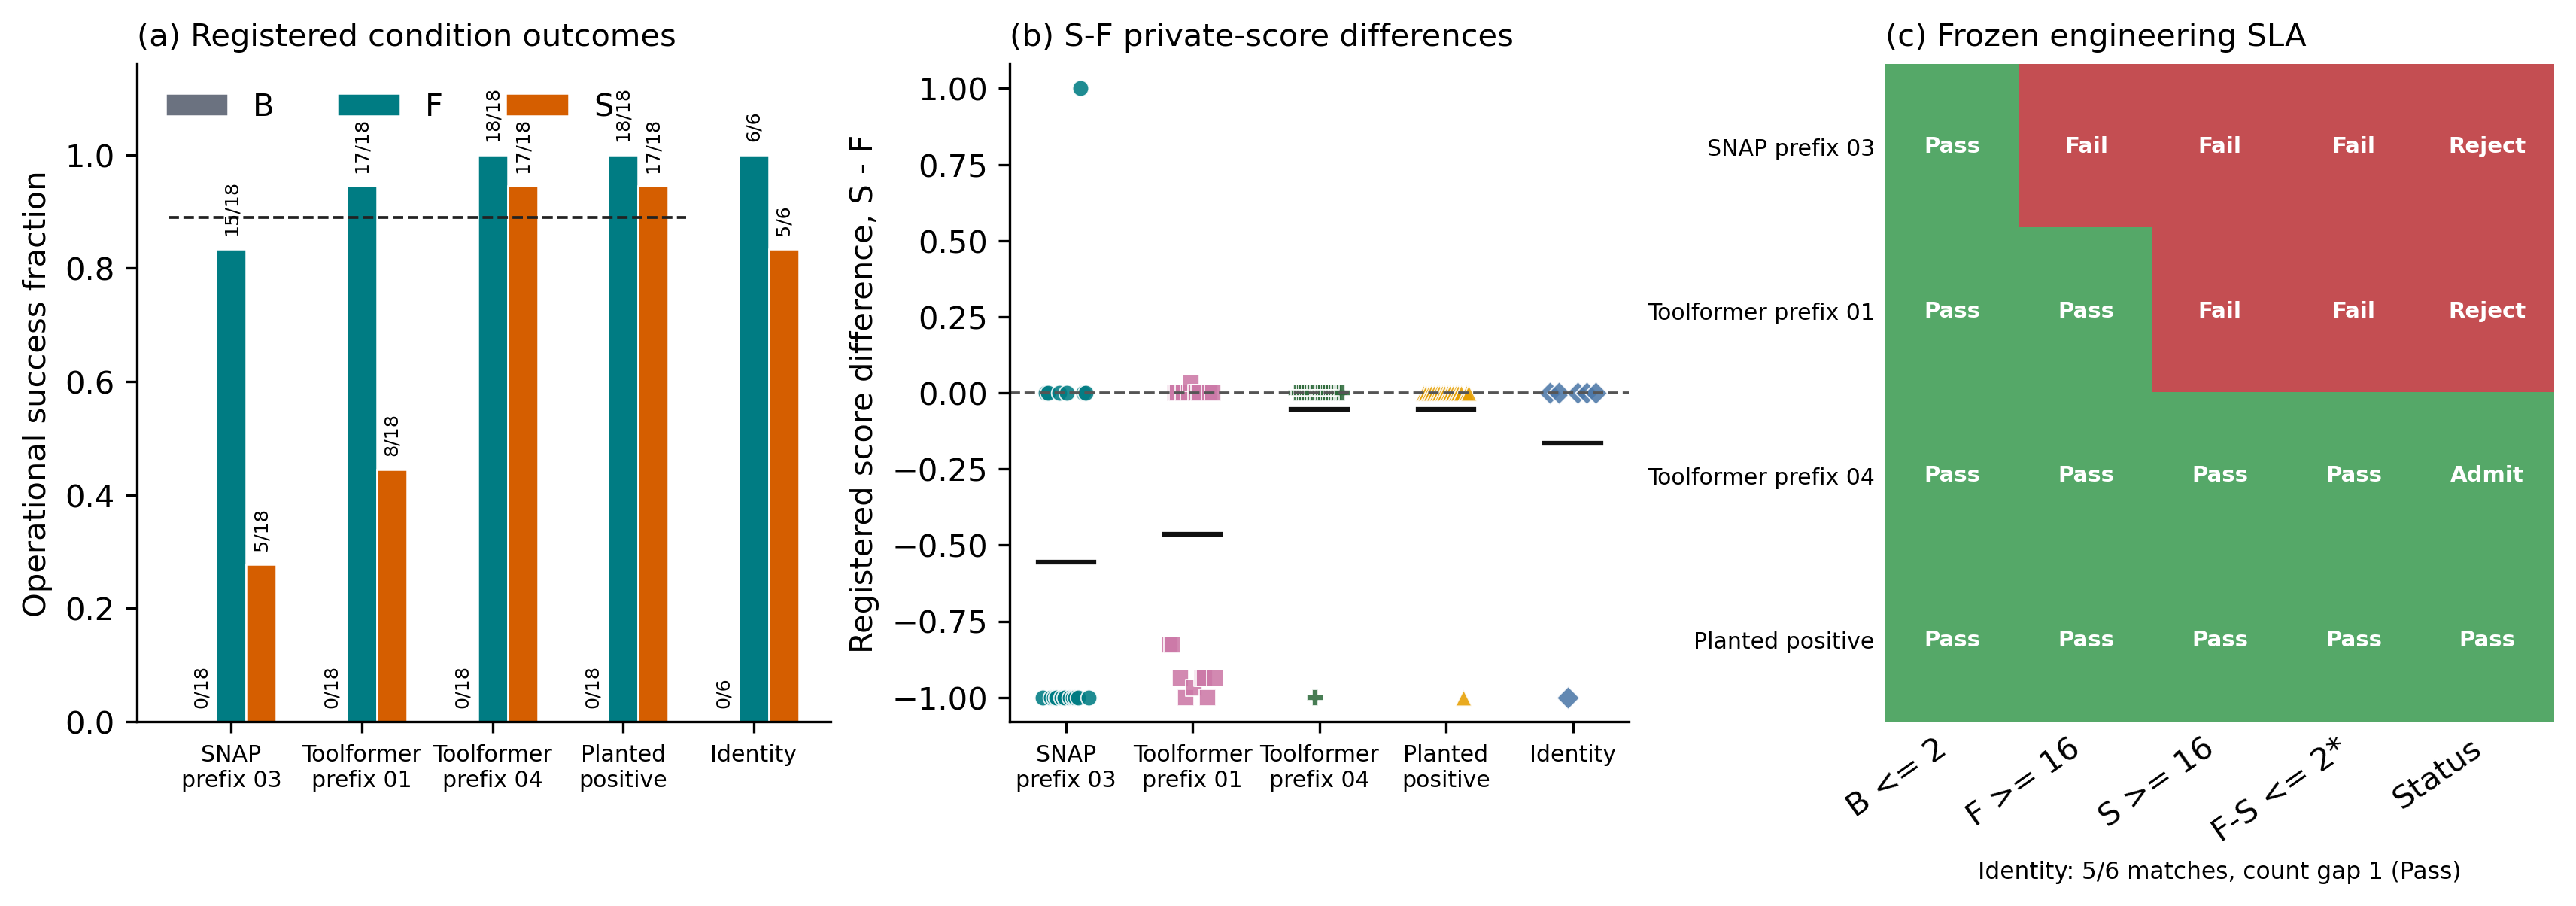
\includegraphics[width=\textwidth]{images/effectslice_v5_finite_schedule.png}
\caption{Focused finite-schedule evidence. (a) Exact operational-success fractions for $B$, $F$, and $S$; the dashed line marks the 16/18 sufficiency threshold for strict-subset families. (b) Every registered block-level $S-F$ private-score difference, with black segments denoting finite-schedule means. (c) Field-level acceptance checks and resulting status. Toolformer prefix 04 was selected after the earlier focused comparison and evaluated on a separately frozen boundary; identity uses its separate paired-agreement rule.}
\label{fig:focused-results}
\end{figure*}

\subsection{RQ2: Decision and Measurement Sanity}

The controls exercise three distinct properties. First, the planted-positive candidate removes only a registered redundant atom and passes at 0/18/17, showing that the gate does not reject every strict subset. Second, the real Toolformer 1/5 negative is rejected at 0/17/8, showing that the same task and scorer can expose a severe omission. Third, byte-identical $F$ and $S$ succeed in 6/6 and 5/6 fresh conversations. Five paired success indicators agree and the aggregate gap is one, so identity instrumentation passes, while the single mismatch demonstrates that identical instructions do not imply identical stochastic trajectories. These controls validate the exercised decision states; they are not a sensitivity/specificity estimate over a population of skills.

The baseline is also essential. A candidate cannot be credited when $B$ already solves the task frequently. In the focused suite, all baseline counts are zero. In the broader stress test, one of the five operational successes occurs under $B$, illustrating why isolated successful rows cannot be interpreted as evidence for the candidate.

\subsection{RQ3: Cross-Paper Scale and Failure Localization}

The cross-paper execution produced all \FGThreeRegisteredRows{} terminal rows. At the primary task level, the frozen analysis yields \FGThreePrimaryRejects{} \textsc{Reject}, \FGThreePrimaryAdmissions{} \textsc{Accept}, and 0 \textsc{Invalid} decisions. Candidate yield is therefore 0/24. This result is not a clean estimate of candidate efficacy: the terminal distribution in Figure~\ref{fig:fg3-failures} is dominated by hard interface and integrity failures. SkillAudit's useful output here is a diagnosis of the evidence boundary, not a claim that all 24 simplified specifications are semantically inadequate.

Only \FGThreeOperationalSuccesses{} individual rows meet the operational-success definition. Table~\ref{tab:five-successes} reports all five. Four are $S$ rows and one is a $B$ row; none is an $F$ row. All have private score 1.0 and pass both hard-contract components. Three successes repeat the same LLMLingua task and model across different blocks. Consequently, these rows do not form matched $B/F/S$ triples, and no defensible $F-S$ effect can be computed from them alone. Reporting a difference would confound artifact condition with task, block, registry, and model.

\begin{table*}[t]
\centering
\small
\setlength{\tabcolsep}{4pt}
\begin{tabular}{lllllrr}
\toprule
Task & Domain & Cond. & Model & Block/registry & Candidate tokens & $q$ \\
\midrule
AGENT-TF-02 & Agent/tool use & $S$ & DeepSeek V3.2 & 3/A & 157 & 1.000 \\
NLP-LLM-01 & NLP & $S$ & GPT-5.6 Sol & 2/A & 170 & 1.000 \\
NLP-LLM-01 & NLP & $S$ & GPT-5.6 Sol & 4/B & 170 & 1.000 \\
NLP-LLM-01 & NLP & $S$ & GPT-5.6 Sol & 5/B & 170 & 1.000 \\
DATA-HDB-01 & Data analysis & $B$ & GPT-5.6 Sol & 2/A & 0 & 1.000 \\
\bottomrule
\end{tabular}
\caption{All operationally successful rows in the 1,296-row cross-paper stress test. These five rows are terminal execution units, not complete task-level comparisons. In particular, their conditions are unbalanced (four $S$, one $B$, zero $F$), so they support protocol diagnosis but not a paired substitution effect.}
\label{tab:five-successes}
\end{table*}

\begin{figure*}[t]
\centering
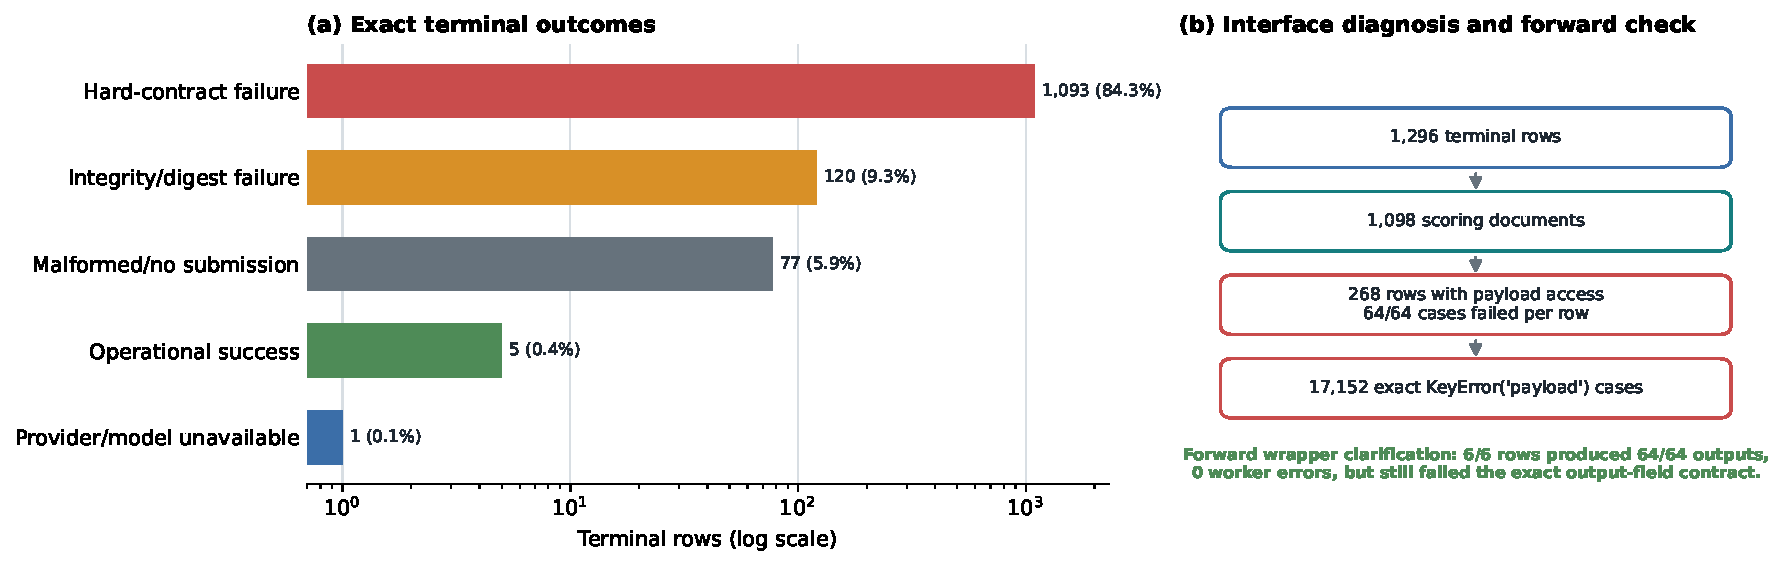
\includegraphics[width=\textwidth]{images/fg3_failure_decomposition.pdf}
\caption{Failure decomposition for the cross-paper stress test. (a) Exact terminal outcomes over 1,296 registered rows; a log axis keeps the five successes and one unavailable-model row visible beside 1,093 hard-contract failures. (b) Interface diagnosis: 268 rows attempted to access a nonexistent outer \texttt{payload} wrapper and failed all 64 private cases, producing 17,152 exact \texttt{KeyError('payload')} cases. A forward wrapper clarification eliminated worker errors in six successor rows, but all six still failed the separately underspecified exact output-field contract.}
\label{fig:fg3-failures}
\end{figure*}

The dominant terminal category is \FGThreeHardContractFailures{} hard-contract failures, followed by \FGThreeIntegrityFailures{} integrity/digest failures, \FGThreeMalformedRows{} malformed or missing submissions, and \FGThreeUnavailableRows{} unavailable-model row. The interface audit reads \FGThreeScoringDocuments{} scoring documents and finds \FGThreePayloadAffectedRows{} affected execution rows with \FGThreePayloadKeyErrors{} exact \texttt{KeyError('payload')} cases. Every affected row fails 64/64 cases, and all 24 task scaffolds are ambiguous about whether \texttt{solve(case)} receives an outer wrapper or its inner payload.

We test this diagnosis with a forward-only interface clarification, without rewriting the 1,296 terminal rows. In six registered successor rows, the task scaffold explicitly states that \texttt{solve(case)} receives the inner payload. All \FGFourForwardRows{} rows then produce \FGFourOutputsPerRow{} outputs with \FGFourWorkerErrors{} worker errors, zero \texttt{KeyError('payload')}, and zero input mutations. They nevertheless receive private score zero because exact output field names remain underspecified. The models return semantically related fields such as \texttt{total\_allocated} or list-valued allocations where the scorer requires \texttt{allocations}, \texttt{by\_name}, and \texttt{total}. This successive localization is precisely why protocol validity and task success must be reported separately.

\subsection{Robustness and Evidence Cost}

Several design choices reduce avoidable confounding. Conditions are interleaved and order-balanced within the focused schedules; starter workspaces are isolated; private cases are terminal; output directories are write-once; and response identifiers, retries, patches, scores, and digests are retained. The cross-paper suite duplicates private registries and varies reducer, retention level, model, and execution family. However, the interface defect prevents those dimensions from serving as a valid model-effect ablation. In particular, the four successes from GPT-5.6 Sol versus one from DeepSeek V3.2 cannot be interpreted as a model ranking.

The focused schedules contain \AllProviderConversations{} conversations, \AllProviderTurns{} provider turns, \AllActions{} recorded actions, and \AllTransportAttempts{} transport attempts. They use \AllInputTokens{} reported input tokens and \AllOutputTokens{} reported output tokens. The cross-paper run invokes a frozen retry policy and records 485 transport retries; only one terminal row remains unavailable. These totals document the cost of evidence generation. SkillAudit does not claim that validation itself is free or that shorter artifacts necessarily reduce end-to-end cost.
